% Chapter Template

\chapter{Related Work} % Main chapter title

\label{Chapter:RelatedWork}

%\subsubsection*{\color{mygray}[Chapter under work]}

%----------------------------------------------------------------------------------------
%	SECTION 1
%----------------------------------------------------------------------------------------

\section{Role of rheological properties in near field electrospun fibers morphology \cite{Flores2017}}

Flores studied SU-8 2002 polymer solutions in cyclopentanone with poly(ethylene) oxide (PEO) and tetrabutylammonium tetrafluoroborate (TBATFB). For that purpose, several samples were prepared with the adequate amounts of PEO and TBATFB with 5 $m l$ of SU-8 2002 and stirred at 160 $r p m$ for one hour at 75 $^\circ C$ in the absence of light. A 5 $m l$ syringe was used to extract the solution from the preparation vial. Finally the syringe was placed upside down for 24 hours to get rid of any bubbles within the solution. Table \ref{tbl:FloresSamples} lists the set of samples that were prepared as values in $w t \%$, dissolved in SU-8 2002.

\begin{table}[th]
\caption{Set of prepared samples}
\begin{center}
\begin{tabular}{ c c c c c c c } 
\hline
\text{} & \multicolumn{2}{c}{Serie A} & \multicolumn{2}{c}{Serie B} & \multicolumn{2}{c}{Serie C} \\
\hline
Sample & PEO & TBATFB & PEO & TBATFB & PEO & TBATFB \\
\hline
1 & 0.00 & 0.00 & 0.00 & 0.50 & 0.50 & 0.00 \\
2 & 0.25 & 0.25 & 0.25 & 0.50 & 0.50 & 0.25 \\
3 & 0.50 & 0.50 & 0.50 & 0.50 & 0.50 & 0.50 \\
4 & 0.75 & 0.75 & 0.75 & 0.50 & 0.50 & 0.75 \\
5 & 1.00 & 1.00 & 1.00 & 0.50 & 0.50 & 1.00 \\
\hline
\label{tbl:FloresSamples}
\end{tabular}
\end{center}
\end{table}

All the samples were executed in a rheometer (Physica MCR 301, Anton Paar) with a cone-and-plane geometry of diameter 24.979 $m m$, angle 4.014$^\circ$ and truncation of 249 $\mu m$. The measurements were performed at a temperature of 25 $\pm$ 0.1 $^\circ C$. For amplitude sweep measurements, the angular frequency was settled at 10 $s^{-1}$, and the percentage amplitude gamma $\% \gamma$, was varied from 0.1 to 1000\%. In flow curve tests, shear rate was applied from 0.1 to 100 $s^{-1}$. For frequency sweeps, the percentage of amplitude gamma, $\% \gamma$, was varied from 0.1 to 100 $s^{-1}$. During the measurements, the rheometer sample area was saturated with cyclopentanone to avoid solvent evaporation.

\subsection{Rheological Characterization : \textbf{Amplitude Sweep}}
The "Serie A`` result measurements indicate that the storage modulus $G'$ is smaller than the loss modulus $G''$. Both moduli have a parabolic behaviour. At low deformation the values of the moduli increase until they become stable at between 1 and 10 $\% \gamma$. After the stabilization, both modulus start to decrease. The increase of PEO and TBATFB concentration $G'$ and $G''$ also increase. Figure \ref{fig:SerieAampSweep} shows the amplitude sweep for the samples of "Serie A``.

\begin{figure}[th]
\centering
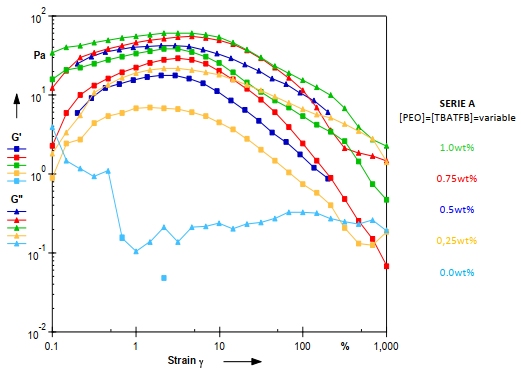
\includegraphics[width=0.75\textwidth]{./Figures/SerieAampSweep.png}
\decoRule
\caption[Serie A - Amplitude Sweep]{Serie A - Amplitude Sweep}
\label{fig:SerieAampSweep}
\end{figure}

The results within Figure \ref{fig:SerieAampSweep} showed that no clear linear viscoelastic region is present. The material has influenced by small deformations, hence it is very sensible to external forces. No yield point was encountered as the moduli separate from each other with the increase of deformation.

Figure \ref{fig:SerieBampSweep} illustrates the results obtained from the amplitude sweeps of Serie B samples. As shown in the figure, the concentration of 0 $w t \%$ shows a constant viscous modulus at 0.2 $Pa$. the 0.25 $w t \%$ concentration sample presented a similar behaviour to the 0 $w t \%$ sample but with a constant value of $G'$ at 2 $Pa$. The other concentrations show a similar parabolic behaviour as the ones in Serie A.

\begin{figure}[th]
\centering
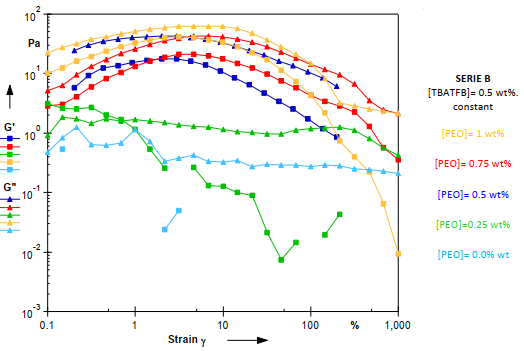
\includegraphics[width=0.75\textwidth]{./Figures/SerieBampSweep.png}
\decoRule
\caption[Serie B - Amplitude Sweep]{Serie B - Amplitude Sweep}
\label{fig:SerieBampSweep}
\end{figure}

\begin{figure}[th]
\centering
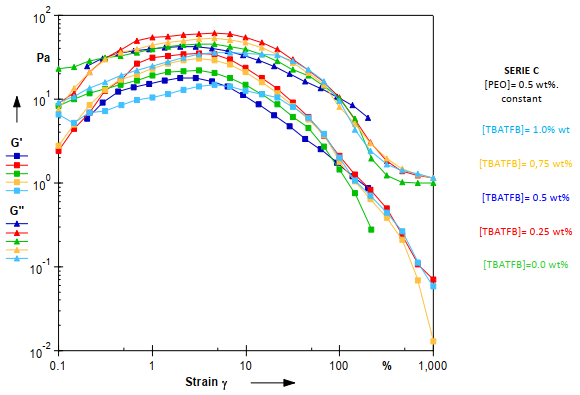
\includegraphics[width=0.75\textwidth]{./Figures/SerieCampSweep.png}
\decoRule
\caption[Serie C - Amplitude Sweep]{Serie C - Amplitude Sweep}
\label{fig:SerieCampSweep}
\end{figure}

The amplitude sweep results of Serie C are depicted in Figure \ref{fig:SerieCampSweep}. Similar to series A and B, results show that the storage modulus $G'$ is smaller than the loss modulus $G''$ with a parabolic behaviour. Typically, the amplitude sweep is to determine the amplitude to be used in frequency sweeps. The amplitude determined by the amplitude sweeps shall keep the material structure undisturbed is known as the linear viscoelastic region (LVER). However, no LVER was found in the samples. For that reason, the percentage of amplitude gamma $\% \gamma$ was found by trial and error. Flores discovered that a $\% \gamma = 20$ has the best performance. 

\subsection{Rheological Characterization : \textbf{Flow Curve}}

Figure \ref{fig:SerieAflowCurve} shows evidence that the equal increase of PEO and TBATFB concentrations result in an increase of shear viscosity rate $\gamma$. for concentrations from 1.00 to 0.25 $w t \%$, a slight increase of flow curve strain $\eta$ for low shear rates to 0.3 $s^{-1}$. For shear rates greater than 0.3 $s^{-1}$, the $\eta$ starts to decrease, as the polymer entanglements start to break apart, reducing friction between the polymer threads and therefore the viscosity also is reduced. The solution samples show a Newtonian-like behaviour and that may be caused by the use of the solvent cyclopentanone and by the small sized SU-8 2002 molecules.

\begin{figure}[th]
\centering
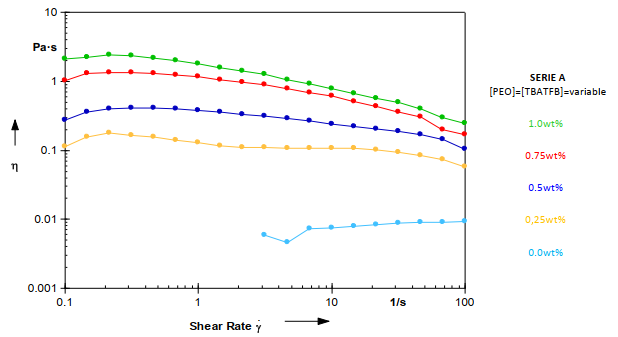
\includegraphics[width=0.75\textwidth]{./Figures/SerieAflowCurve.png}
\decoRule
\caption[Serie A - Flow curve]{Serie A - Flow curve}
\label{fig:SerieAflowCurve}
\end{figure}

From the results in Figure \ref{fig:SerieAflowCurve}, it is noticeable that the addition of small amounts of PEO and TBATFB cause a change of one order of magnitude in shear viscosity in small concentration and a triple change in high concentrations.

Series B flow curve results (Figure \ref{fig:SerieBflowCurve}) do not show a clear correlation between PEO concentrations and shear viscosity. For PEO of 1 $w t \%$, a slow increase in $\eta$ is present with the increase of shear rate, after $\gamma$ drops from 2 to 0.8 $Pa s$, a shear thinning behaviour is present. For 0.50 and 0.75 $w t \%$ concentrations, a shear thinning behaviour is present throughout the plot. For the 0.50 $w t \%$ sample, viscosity value varied between 0.2 and 0.4 $Pa s$; and between 0.5 and 2.0 $Pa s$ for the 0.75 $w t \%$ sample. Viscosity is stabilized at 0.1 $Pa s$ when the shear rate is between 1 and 20 \% for the sample of PEO $w t \%$. After stabilization, the viscosity decreases from 0.1 to 0.02 $Pa s$ for shear rates between 20 to 100 $s^{-1}$. For PEO 0.00 $w t \%$, a high variation is present in viscosity readings due to the presence of electrolytes cause amendments in the polymer chain within the solution.

\begin{figure}[th]
\centering
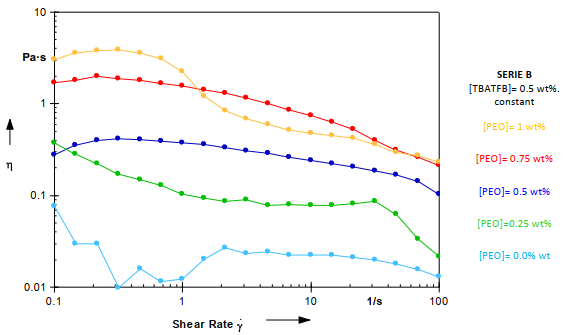
\includegraphics[width=0.75\textwidth]{./Figures/SerieBflowCurve.png}
\decoRule
\caption[Serie B - Flow curve]{Serie B - Flow curve}
\label{fig:SerieBflowCurve}
\end{figure}

The flow curve results of Serie C are presented in Figure \ref{fig:SerieCflowCurve}. The sample with 1 $w t \%$ TBATFB concentration shows a shear thinning behaviour for shear rates varying between 0.1 to 15 $s^{-1}$. The 1 $w t \%$ sample describes a drop in viscosity for shear rates between 15 to 20 $s^{-1}$ followed by a stable state. A similar behaviour is observed for concentration of 0.75 $w t \%$. and less evident for 0.0 $w t \%$. For concentrations of 0.5 $w t \%$ and 0.25 $w t \%$ the behaviour of the shear viscosity is similar.

\begin{figure}[th]
\centering
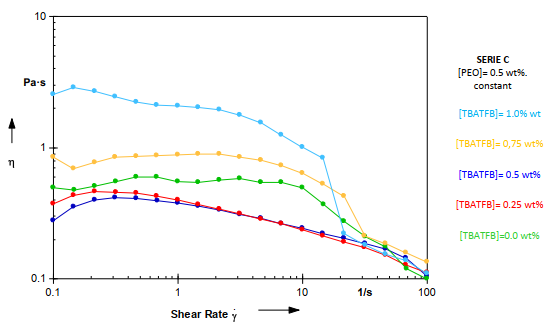
\includegraphics[width=0.75\textwidth]{./Figures/SerieCflowCurve.png}
\decoRule
\caption[Serie C - Flow curve]{Serie C - Flow curve}
\label{fig:SerieCflowCurve}
\end{figure}

\subsection{Rheological Characterization : \textbf{Frequency Sweep}}



\clearpage

\section{Advanced Manufacturing Techniques for the Fabrication and Surface Modification of Carbon Nanowires \cite{Cardenas2017}}


%-----------------------------------
%	SUBSECTION 1
%-----------------------------------


